\section{Started Service}
Started Service는 Context의 startService() 메서드를 통해서 시작된다. 이것 역시 startService()를 호출하는 시점에 Service가 바로 시작되는 것이 아니고, 메인 Looper MessageQueue에 들어가서 메인 스레드를 쓸 수 있는 시점에 Service가 시작된다. startService() 메서드는 곧바로 ComponentName을 리턴하고 다음 라인을 진행한다. startService()는 Intent Bundle에 파라미터를 전달하고 Service에 작업을 하도록 요청해놓는 것 뿐이다.\\

Service는 startService() 메서드를 통해 처음 생성되는 경우에는 onCreate 메서드를 거쳐서 onStartCommand() 메서드를 실행하며, 그 이후에 startService()를 실행할 때면 onCreate() 메서드는 거치지 않고 onStartCommand() 메서드가 실행된다.
onCreate() 메서드 역할은 Service에 필요한 리소스 등을 준비해 놓은 작업을 하고, onStartCommand() 메서드 역할은 이름 그대로 명령을 매번 처리하는 것이다. 그래서 Activity와는 다르게 onCreate() 메서드에는 Intent가 전달되지 않는다.\\

\begin{comment}
쉬운 이해를 위해서, 비유를 들어 얘기해보자.\\
장난감 회사에 홍보 부서를 만들기로 했다.(이것이 Manifest에 등록된 Service이다.). 홍보할 것이 없으면 딱히 할 것도 없이 가만히 있는다. 그러다가 `로보카 폴리 홍보'라는 의뢰가 들어온다.(이것이 startService이다. 의뢰 내용이 Intent이다). 미리 리소스를 준비해놓지 않고 있다가 그제서야 부서를 만들고 복사기나 사무집기 등을 준비한다.(이것을 onCreate라고 봐도 된다.) 그리고서 의뢰 내용을 회의 등을 거쳐서 처리한다.(이것이 onStartCommand 이다). 이제 다른 의뢰가 들어오면 이제는 의뢰 내용만 처리하면 된다.(onStartCommand만 실행한다.)\\
\end{comment}

명령을 던져놓고 Service에서 그 명령을 알아서 실행하는 것에 Started Service를 사용한다고 생각하자.
표준 패턴은 onStartCommand()에서 백그라운드 스레드를 생성해서
백그라운드 상에서 작업을 진행하고, onStartCommand()를 바로 리턴한다. 이런 패턴을 알지 못하고서 필자가 처음 앱을 개발할 때 겪은 문제도 있다. Service에 명령을 보내고서 화면에 작업중이라는 표시의 애니메이션을 실행하고, 작업이 끝나면 애니메이션을 중지하는 기능이다. 
그런데 Service의  onStartCommand() 메서드에서 스레드를 사용하지 않고 작업을 진행해서 메인 스레드를 점유하고 있으니, 역시 메인 스레드를 사용하는 애니메이션이 동작할 리가 없었다. 원리를 이해하면 아무 것도 아니지만 당시에는 당황했던 기억이 있다.\\

Service에서 작업 진행 상황에 따라 Activity에 메시지를 보내려고 한다면 일반적으로 Broadcast를 사용한다.
예를 들어, 서버와 동기화를 하는 SyncService가 있고 화면에서 버튼이나 메뉴로 SyncService를 시작한다. 
동기화를 하는 도중에는 ProgressBar로 `진행중'을 표시하고 동기화가 끝날 때는 ProgressBar를 없애고 종료 메시지를 표시하고자 한다.
이때 Activity에서는 BroadcastReceiver를 등록하고 Service에서는 sendBroadcast()를 실행하는 식이다.\\

또 다른 방식으로는 Intent에 ResultReceiver를 전달하고 Service에서 ResultReceiver에 값을 되돌려줄 수도 있다. 단방향 메시지 전달이라면 이 방식이 간편하다.\\

ResultReceiver 사용 샘플은 아래와 같다. 먼저 Activity의 내용을 보자. 
\begin{lstlisting}[frame=single]
	private View syncLayout, progressBar;
	private TextView syncMessage;

	@Override
	protected void onCreate(Bundle savedInstanceState) {
   		super.onCreate(savedInstanceState);
   		setContentView(R.layout.data_sync);
   		syncLayout = findViewById(R.id.sync_layout);
   		progressBar = findViewById(R.id.progress_bar);
  	 	syncMessage = (TextView) findViewById(R.id.sync_message);
	}

	public void onClickSync(View view) { // (1)
   		syncLayout.setVisibility(View.VISIBLE);
   		progressBar.setVisibility(View.VISIBLE);
   		syncMessage.setText(R.string.sync_progress);

   		Intent intent = new Intent(this, SyncService.class);
   		intent.putExtra(Constant.EXTRA_RECEIVER, resultReceiver); // (2)
   		startService(intent);
	}

	private Handler handler = new Handler();

	private ResultReceiver resultReceiver = new ResultReceiver(handler) { // (3)

   		@Override
   		protected void onReceiveResult(int resultCode, Bundle resultData) {
      		if (resultCode == Constant.SYNC_COMPLETED) { // (4)
         		progressBar.setVisibility(View.GONE);
        		syncMessage.setText(R.string.sync_ended); 
      		}
  		 }

	};	
\end{lstlisting}
\begin{itemize}
\item 13라인(1)의 onClickSync() 메서드가 `동기화' 버튼을 클릭할 때 동작이다. 동기화 관련 레이아웃과 ProgressBar를 visible 상태로 변경하고 텍스트 메시지도  R.string.sync\_progress로 보여준다.
\item 25라인(3)에서 ResultReceiver를 생성하고 ResultReceiver에는 비어 있는 메서드인 onReceiveResult() 메서드를 오버라이드한다. 
\item 29라인(4)에서 SYNC\_COMPLETED resultCode를 받으면 ProgressBar를 감추고 텍스트 메시지는 R.string.sync\_ended로 변경한다. 
\item 25라인(3)의 ResultReceiver 생성자에는 Handler를 넣기도 하고 null로 할 수도 있다. Service의 백그라운드 스레드에서 ResultReceiver의 send() 메시지를 호출하는데, 여기서 UI를 업데이트하기 때문에 Handler를 거쳐 메인 Looper MessageQueue에 넣은 것이다. 호출하는 쪽과 받는 쪽이 둘다 백그라운드 스레드에서 동작한다면 null을 사용해도 된다.
\item 19라인(2)에서 Intent Extra에 ResultReceiver 인스턴스를 전달한다. ResultReceiver는 Parcelable을 구현해서 다른 프로세스 간에도 데이터를 주고받을 수 있는 구조이다.
\end{itemize}

이제 Service에서 ResultReceiver를 사용하는  소스를 보자.
\begin{lstlisting}[frame=single]
	@Override
	public int onStartCommand(Intent intent, int flags, int startId) {
   		new Thread(new Runnable() {
      
      		@Override
     		public void run() {
         		Log.d(TAG, "SyncService started");
         		SystemClock.sleep(10000);
         		final ResultReceiver receiver 
         			= intent.getParcelableExtra(Constant.EXTRA_RECEIVER); // (1)
         		receiver.send(Constant.SYNC_COMPLETED, null); // (2)
         		stopSelf();
     		}

   		}).start();
   
   		return START_NOT_STICKY;
	}
\end{lstlisting}	
10라인(1)에서 Intent에서 ResultReceiver를 꺼내오고, 작업을 다한 후에 11라인(2)에서 send() 메서드를 호출해서 SYNC\_COMPLETED라는 결과를 다시 보낸다. 여기서는 메시지를 하나만 보냈지만 작업 진행률이나 실패 메시지와 같은 다양한 결과를 보낼 수 있을 것이다.

\subsection{Service 재시작 방식}
가용 메모리가 낮고 포커스를 갖고 있는 Activity의 시스템 리소스를 복구해야 할 때, 안드로이드 시스템은 Service를 강제 종료시키기도 한다. 
그리고서 가능한 한 빨리 Service를 재시작하는데, 여기서 Started Service를 사용하면서 주의할 부분이 있다.
Service도 우선순위에 따라 언제든지 종료될 수 있는데 시스템이 알아서 재시작한다는 의미에서 Service를 믿고 안정감을 얻을 수도 있지만, 방식을 이해하지 않으면 반복해서 크래시를 맞이할 수도 있다.\\

Started Service에서는 onStartCommand() 메서드에서 리턴하는 int 상수를 가지고서 재시작 방식을 제어한다. onStartCommand() 메서드의 시그너처는 다음과 같다.\\

public int onStartCommand(Intent intent, int flags, int startId)\\

리턴값으로 사용되는 int 상수를 하나씩 살펴보자.\\
\underline{\bfseries START\_NOT\_STICKY} startService()를 통해서 onStartedCommand() 메서드가 리턴된 상태에서 kill 되면 재시작하지 않는다. 명시적으로 startService()를 실행할 때만 의미가 있는 작업에 사용한다.
예를 들어, 화면에 보여줄 뉴스를 네트워크를 통해서 가져와서 저장할 수 있는데, 메모리 이슈로 인해 Service가 kill되었다면 다시 startService() 명령을 기다려서 최신 뉴스를 가져오는 것이 나을 것이다.\\

\underline{\bfseries START\_STICKY} onStartCommand() 메서드의 기본 리턴 값이다. 정상적으로 종료되지 않았을 때 재시작한다. 재시작시에는 다시 onStartCommand()를 호출하는데 이때 Intent 매개변수가 null로 전달된다.
startService()를 실행할 때 Intent에 값을 전달하고 이 값을 startCommand() 메서드에서 사용할 때는 NullPointerException 발생 가능성이 있다. 
전달된 Intent 값을 사용하지 않고 내부적인 상태만을 가지는 Service에 적합하다.
예를 들면 서버 API 에 접근해서 날씨 정보를 가져와서 업데이트하는 것과 같이 지속적인 데이터 동기화 작업이 해당한다.\\

\underline{\bfseries START\_REDELIVER\_INTENT} 재시작하면서 onStartCommand()에 Intent를 다시 전달하여 실행한다. 어떻게든 해당 파라미터를 가지고 실행해야 하는 Service가 이에 해당한다. 쇼핑몰 앱에서 API를 통해서 회사의 상품 목록을 가져온 후 DB에 저장하는 경우를 예로 들 수 있다.\\

재시작 제어 방식도 중요하지만 불필요한 재시작이 발생하는 상황을 없애는 것도 중요하다. 재시작이 안 되려면 정상적인 종료라는 조건이 필요하다. 
Service를 종료하는 방법으로 Context에 stopService() 메서드가 있지만 실제 사용 빈도가 크지 않다. 
앱을 사용하는 내내 실행되는 Service라면 모르지만, 그런 케이스가 많지 않고 권장되는 방식도 아니다. 
Service는 필요할 때만 동작하고 종료하는 것이 좋다.
그럼 Service를 정상 종료하기 위해서 어떤 것을 주로 사용하는가 하면, 바로 Service의 stopSelf() 메서드를 사용한다. 
stopSelf() 메서드는 stopService() 메서드와 역할이 동일하지만 Service 내에서 호출한다는 것이 다를 뿐이다. Service에서 할 일이 다 끝났으면 (백그라운드 스레드든 아니든) stopSelf()를 실행해서 Service를 명시적으로 종료하고 이때 Service는 onDestroy()까지 실행된다.\\

만일 stopSelf()를 실행하지 않은 상태로 계속 남아있다면 어떤 일이 벌어질까. 할 일은 다 끝났는데 Service는 불필요하게 메모리를 차지하고 있고 시작된(started) 상태로 남아있다. 
어느 순간에 메모리 이슈로 Service가 kill되면 리턴 상수가 START\_STICKY나 START\_REDELIVER\_INTENT인 경우에 의도치 않게 재시작하는 일이 생긴다.

\subsection{멀티 스레드 이슈}
Started Service에서 주의할 게 더 있다. 바로 멀티 스레드 이슈이다. 여러 곳에서 startService()를 동시에 호출할 수 있다. 
그래도 어차피 UI 스레드는 단일 스레드 모델이므로, onCreate(), onStartCommand() 메서드는 한번에 하나씩만 호출된다.
그런데 onStartCommand()에서 백그라운드 스레드를 여러 개 동시에 실행할 때, 값을 잘못 공유하면 문제 발생 여지가 생긴다. 앞에서 예를 든 쇼핑몰 앱에서 각 회사마다 API를 통해 상품 정보를 가져오는데, 전달된 Intent의 회사 id를 Service의 멤버 변수로 쓰면 어떤 일이 벌어질까? 바로 엉뚱한 곳에 데이터가 저장되는 상황을 맞게 된다.\\

여러 클라이언트에서 startService()를 실행한다면 각각 작업이 끝났을 때 아직 진행중인 것이 있는지 알 수 없는 경우도 있다. 이때 stopSelf() 메서드를 호출하면 진행중인 작업들에서 문제가 발생한다. 
이 경우에 대비해서 stopSelf() 메서드의 변종인 stopSelfResult(int startId) 메서드가 있다.  startId는 onStartCommand()에서 전달된 값으로 이 startId가 가장 최근에 시작된 것이라면 Service를 종료한다. 이 메서드를 사용하면 각각의 작업이 끝날 때마다 stopSelfResult()를 실행해도 더 안전해진다.

\subsection{암시적 인텐트로 서비스 실행}
Service는 AndroidManifest.xml에 등록할 때 intent-filter를 추가하면 외부에서 접근할 수 있다.
\begin{lstlisting}[frame=single]
<service android:name=".app.RemoteService" android:process=":remote">
	<intent-filter>
		<action android:name="com.example.android.apis.app.REMOTE_SERVICE" />
	</intent-filter>
</service>
\end{lstlisting}

\begin{lstlisting}[frame=single]
ComponentName componentName = startService(new Intent("com.example.android.apis.app.REMOTE_SERVICE"));
\end{lstlisting}
action name이 동일한 Service가 여러 개 있는 경우는 어떨까? 참고로 Activity의 경우는 action name이 동일하면 Activity를 선택하라는 화면을 보여주고, Broadcast는 action name이 동일한 모든 BroadcastReceiver를 실행한다.
Service는 intent-filter의 android:priority 속성값\footnote{\url{http://developer.android.com/guide/topics/manifest/intent-filter-element.html}를 참고하자. priority값은 -999에서 999까지이다. 디폴트값은 0이다. 실제로 범위를 넘는 값을 넣어도 실행에는 문제가 없다. IntentFilter 소스를 봐도 체크 로직이 없다. 가용한 범위도 충분하기 때문에 굳이 범위를 넘어서 쓰진 말자. 이후 버전에서는 유효성 체크에 범위가 사용될 수도 있다.}을 먼저 비교해서 높은 것을 실행하고, android:priority 값이 같은 경우에는 시스템이 랜덤으로 선택해서 실행한다.

\begin{lstlisting}[frame=single]
<service android:name=".app.RemoteService" android:process=":remote">
	<intent-filter android:priority="999">
		<action android:name="com.example.android.apis.app.REMOTE_SERVICE" />
	</intent-filter>
</service>
\end{lstlisting}

intent-filter를 적용하지 않고 외부에서 서비스를 직접 시작할 수도 있다. 바로 명시적 인텐트를 사용하는 것이다.
\begin{lstlisting}[frame=single]
ComponentName cName = new ComponentName("com.example.android.apis",
	"com.example.android.apis.app.ServiceStartArguments");
startService(new Intent().setComponent(cName));
\end{lstlisting}

여기에는 제약사항이 있다. 바로 AndroidManifest.xml에 android:exported 속성을 true로 줘야 한다.\footnote{android:exported 속성은 false이고 intent-filter가 있다면 디폴트값이 true가 된다.}
\begin{lstlisting}[frame=single]
<service android:name=".app.ServiceStartArguments" android:exported="true" />
\end{lstlisting}

롤리팝부터는 암시적 인텐트로 Service를 시작하면 문제가 발생한다. startService(), bindeService() 둘 다 마찬가지다.
AndroidManifest.xml에 targetSdkVersion을 21이상으로 하면 롤리팝 이상 단말에서 `java.lang.IllegalArgu\-mentException: Service Intent must be explicit'  예외가 발생하고, targetSdkVersion이 그 아래이면 호환 모드로 동작하여 예외가 발생하진 않지만 `W/ContextImpl: Implicit intents with startService are not safe: Intent { act=com.naver.android.sample.SYNC\_SERVICE (has extras) } android.content.ContextWrapper.startService:533 ...'과 같은 로그가 남는다. 
관련해서 코드를 보려면 롤리팝 버전 ContextImpl의 validateServiceIntent() 메서드를 보자. 여기서도 targetSdkVersion을 체크하는 것을 볼 수 있다.\\

만일 클래스명을 알고 있다면 롤리팝에서도 앞에서 ComponentName을 쓴 것처럼 명시적 인텐트를 사용하면 된다.

\subsection{IntentService}
일반적인 앱에서 멀티 스레딩이 필요한 경우가 많지는 않다. 동시에 여러 요청을 처리할 필요가 없다면 IntentService를 활용하자.
IntentService는 내부적으로 1개의 백그라운드 스레드를 두고 전달된 Intent를 순차적으로 처리한다(내부적으로 HandlerThread를 사용한다).\\

IntentService에서는 백그라운드 스레드에서 실행되는 내용인 onHandleIntent(Intent) 메서드만 구현하면 된다.
물론 생성자 문제 때문에 한 가지를 더 해야 한다. 아래와 같이 생성자가 추가되지 않으면 `no empty constructor exception'이 발생한다. 
\begin{lstlisting}[frame=single]
public class NewsReaderService extends IntentService {

	public NewsReaderService() {
		super("NewsReader");
	}

	@Override
	protected void onHandleIntent(Intent intent) {
		...
	}
	
}	
\end{lstlisting}
IntentService에서 내부적으로 구현한 onStartCommand() 메서드는 기본 리턴값은 START\_NOT\_STICKY이다. 이 값을 변경하려면 생성자에서 아래 메서드를 호출하면 된다.\\ 

setIntentRedelivery(true)\\

IntentService를 사용할 때 내부 구조를 이해하지 못하면 생기는 문제가 있다. 
한 예를 들어보자.\\

백그라운드 스레드에서 Toast를 띄우려고 하면, Toast 내부 클래스 TN에서 new Handler()로 Hanlder 생정자를 사용하는 부분이 있어서 Looper가 없다고 에러를 발생시킨다. 그럼 백그라운드 스레드에서 Looper.prepare()를 실행하면 어떤가 하면 Toast를 정상적으로 보여준다.\\

그럼 IntentService의 작업 스레드에서 동작하는 메서드인 onHandleIntent()에서 Toast를 띄운다면 어떨까. 
내부적으로 사용하는 HandlerThread에서 이미 Looper.prepare()가 되어 있기 때문에 Toast가 뜨는 게 문제없어 보이고, 여기서 크래시가 나진 않지만 심각한 오동작이 가끔 발생한다.\\

Toast.show()를 실행하면 Binder 통신을 통해 system\_server 프로세스에서 NotificationManagerService의 enqueToast() 메서드를 호출한다. 이때 파라미터로 Binder Callback(TN 인스턴스)이 전달되고, Callback에서는 화면에 Toast를 보여주는 작업과 일정시간 후에(Toast.LENGTH\_SHORT, Toast.LENGTH\_LONG) 제거하는 작업을 진행한다.\\

그런데 IntentService에서는 onHandleIntent() 실행 이후에 바로 stopSelf()를 호출하고, onDestroy()에서는 HandlerThread에서 생성한 Looper를 종료하는 Looper.quit()을 호출한다. Looper가 종료되면서 생기는 현상은 Looper의 MessageQueue에 전달되는 Callback이 실행되지 않는다는 것이다.
이때 크래시는 나지 않고 로그에 MessageQueue 태그로 Warning이 나온다. `... sending message to a Handler on a dead thread'\\

뜨기로 한 Toast가 안 뜨는 건 해로운 정도는 아니다. 문제는 실행 시점 때문에 Toast는 떴지만, Toast 제거하는 Callback이 불리지 않는 것이다(중간에 Looper가 종료된 것이다).
Toast가 사라지지 않고 내내 남아있는 현상이 발생하는데 심각한 문제다. 그런데 이게 결국 시점 문제라서 재현이 잘 되지도 않는데, 결국 원리를 모르면 해결할 수 없는 문제가 되고 만다.\\

Toast는 가급적 메인 스레드에서만 띄우는 게 맞다. 백그라운드 스레드에서는 그냥 쓰면 크래시가 나기 때문에 결국 안 쓰게 되지만, IntentService에서 아무 고려 없이 `써보니 잘 되네' 하고 넘어가면 안 된다. Looper.getMainLooper()를 통해 메인 스레드에 연결된 Handler를 가지고서 Toast를 띄우는 것이 더 적절하다.
%간단 샘플 필요

\subsection{Service 중복 실행 방지}
코드 \ref{SleepService}에서는 onStartCommand()가 아닌 onCreate() 에서 스레드를 생성해서 작업을 처리하였다. 
이렇게 한 의도는 여러 곳에서 startService()를 실행하는 경우에도 매번 실행하지 않고, 이미 시작되었으면 나머지는 skip하려는 의도를 가지고 만들어 본 것이다.
skip이 필요한 경우를 얘기해 보자. 
메모 앱 같은 경우 시작할 때도 동기화를 실행하고, 버튼을 눌러도 동기화를 실행하고, 메모를 추가했을 때도 동기화를 실행하려고 한다. 
그런데 동기화 작업같은 경우 동시에 여러 개를 실행하면 문제 발생 소지가 있다. 
앱 사용자는 이런 작업이 하나씩 끝날 때까지 대기하는 것이 아니기 때문에, 하다보면 여러 곳에서 시간이 겹친 채로 동기화를 실행할 수 있다.
이때 한가지 작업에만 충실하고 나머지는 확실히 skip해야 하는데, 코드 \ref{SleepService}처럼 onCreate()에서 처리하는 방법도 가능하다. 
onCreate()는 처음 startService()를 호출할 때만 실행하기 때문이다. 
작업이 끝나면 확실히 stopSelf()를 호출한다면 문제가 없다. 다만 Service의 본래 사용 방식과 차이가 있다.\\

IntentService가 skip 용도에 맞는 게 아닐까 하는 생각을 할 수도 있는데, 
IntentService는 백그라운드 스레드 Looper의 MessageQueue에 넣고 순차적으로 하나씩 실행하는 것이므로 이 의도에는 맞지 않다. 여러 번 동기화를 `순차적으로' 실행하는 셈이 된다.\\

onCreate() 메서드가 아닌 onStartCommand() 메서드에서 이런 skip 방식을 적용한 샘플을 보도록 하자.
\begin{lstlisting}[frame=single]
public class SleepThreadService extends Service {

	private static final long SLEEP_TIME = 10000;
	
	private ExecutorService exec = Executors.newSingleThreadExecutor();
	
	@Override
	public void onCreate() {
		Log.d("suribada", "Service onCreate");
	}
	
	private boolean isRunning = false;
	
	@Override
	public int onStartCommand(Intent intent, int flags, int startId) {
		if (isRunning) {
			Log.d("suribada", "skip");
			return START_NOT_STICKY;
		}
		isRunning = true;
		exec.submit(new Runnable() {

			@Override
			public void run() {
				Log.d("suribada", "Thread start");
				SystemClock.sleep(SLEEP_TIME);
				Log.d("suribada", "10 seconds after");
				SystemClock.sleep(SLEEP_TIME);
				Log.d("suribada", "20 seconds after");
				SystemClock.sleep(SLEEP_TIME);
				Log.d("suribada", "30 seconds after");
				stopSelf();
			}
		});
		return START_STICKY;
	}
	
	@Override
	public void onDestroy() {
		isRunning = false;
	}
	
	@Override
	public IBinder onBind(Intent intent) {
		return null;
	}

}
\end{lstlisting}
onStartCommand()는 메인 스레드에서 동작하기 때문에 단순한 boolean 값 가지고 체크가 가능하다.
skip 시에는 START\_NOT\_STICKY를 리턴하는 것도 기억하도록 하자.\\

자바의 concurrency 패키지를 사용한다면 TheadPoolExecutor를 직접 쓰는 방식도 가능하다. 위에서 사용한 Executors.newSingleThreadExecutor() 메서드 같은 정적 메서드는 일반적으로 많이 사용되는 TheadPoolExecutor를 팩토리 메서드로 만든 것이다.\\

ThreadPoolExecutor에 스레드 개수를 1로 고정하면 스레드 풀에 하나의 스레드만 사용하는데, 여기서 중요한 것은 마지막에 추가된 DiscardPolicy이다. 추가로 요청이 들어온다면 버리는 동작을 하는 것이다.
% 만일 이 값이 따로 없다면 crash
\begin{lstlisting}[frame=single]
public class SleepThreadService extends Service {
	
	private ThreadPoolExecutor exec = new ThreadPoolExecutor(1, 1, 
		0, TimeUnit.SECONDS, new SynchronousQueue<Runnable>(), 
		new ThreadPoolExecutor.DiscardPolicy());	
	....
		
	@Override
	public int onStartCommand(Intent intent, int flags, int startId) {
		exec.submit(new Runnable() {

			@Override
			public void run() {
				....
				stopSelf();
			}
		});
		return START_STICKY;
	}
	
	....

} 
\end{lstlisting}

\section{Bound Service}
Bound Service는 Service에서 제공하는 메서드를 다른 컴포넌트에서 호출할 수 있게 한 것으로 사용 절차는 간단하다. 먼저 bindService() 메서드를 실행해서 Binding된 이후에 필요한 메서드를 실행한다.\\

Context 클래스에 있는 bindService()의 메서드 시그너처는 아래와 같다.\\
public abstract boolean  bindService (Intent service, ServiceConnection conn, int flags)\\
\begin{itemize}
\item 첫 번째 파라미터인 service는 대상 Service를 가리킨다.
\item 두 번째 파라미터인 conn은 Service에 연결되고 연결이 끊길 때의 Callback이다.
\item 세 번째 파라미터인 flags에는 0을 넣을 수도 있고, Context의 BIND\_XXX 상수를 비트합으로 넣을 수도 있다. ICS부터 추가된 상수들은 주로 Service 프로세스의 우선순위와 관련된 것이고, 가장 많이 쓰이는 상수는 Context.BIND\_AUTO\_CREATE이다.\\

BIND\_AUTO\_CREATE을 쓸 때만 bindService()를 실행할 때 Service가 없다면 새로 Service를 생성한다. 이 옵션이 없다면 어디선가 startService()를 하지 않았다면 bindService()에서 연결 Callback이 불리지 않게 된다.
즉 Started \& Bound Service가 아니라면 BIND\_AUTO\_CREATE 옵션은 필수적이다. 
이 옵션의 역할은 그 밖에도 더 있다. 
Service에 Binding된 클라이언트가 여러 개 있을 때 stopService()를 실행하면 어떤 일이 발생할까? 이 옵션이 있다면 stopService()를 실행해도 Service가 종료되지 않는데, 옵션이 없는 경우에는 연결이 끊기고서 바로 Service의 onDestroy()가 불린다.
옵션이 있는 경우 unbindService()를 클라이언트마다 모두 실행해야 Service의 onDestroy()가 불린다.
Binding된 Client가 남아 있다면 Service 프로세스가 메모리 문제 등으로 종료되었다가도 다시 Service 프로세스가 살아나나서 재연결되는 것도 이 옵션이 있을 때만 가능한다. 
\end{itemize}

Bound Service의 용도를 이제 생각해보자.
최신 뉴스나 인기검색어, 날씨처럼 업데이트가 필수적인 데이터가 있다. 이런 데이터를 앱에서 쓰는 방법은 어떤 게 있을까?
\begin{enumerate}
\item XML이나 JSON으로 데이터를 리턴하는 API 서버를 만들고, 앱에서 HTTP 호출을 통해 데이터에 접근한다.
\item HTTP 호출을 하고 결과도 객체로 리턴해주는 오픈 API jar를 만들어서, 앱에서는 jar를 이용해서 데이터에 접근한다.
\item 서비스 앱에서 데이터를 제공하는 Bound Service를 만들고(이 안에서 HTTP 호출을 하고 객체를 리턴한다), 다른 앱에서는 bindService()를 실행하여 Service 데이터에 접근한다. 이를테면 검색 앱에서는 인기검색어 목록을 Bound Service로 외부에 제공할 수 있다.
Google Play In-app Billing도 이 방식을 사용하고 있다.
\item bindService()를 실행하고 결과를 받는 것을 래핑한 jar를 만들어서, 다른 앱에서 이 jar를 이용한다. Google Play Services(\url{https://developers.google.com/android/guides/overview})가 이런 형태이다.\footnote{connect()와 disconnect() 메서드가 있는데, bindService()와 unbindService()를 내부적으로 호출해서 사용한다.}
\end{enumerate}
3번과 4번에서 Bound Service를 언급하였다. 
아래로 갈수록 추상화 레벨이 높다. 추상화 레벨이 높은 게 좋은 게 아니라, 현재 시점에 맞는 적절한 방법을 선택하는 게 좋겠다. 오버 엔지니어링을 피하자는 얘기다.\\

Bound Service는 구분해서 로컬 바인딩(Local Binding)과 리모트 바인딩(Remote Binding) 2가지를 얘기한다.
혹자는 뭐하러 Local과 Remote를 구분하느냐고 말하기도 한다.
Remote Binding Service를 만들어도, 로컬에서 호출하면 Binder를 거치지 않고 직접 호출하므로 Local Binding Service가 따로 있을 필요가 없다는 것이다. Remote Binding만으로 커버 가능한데, 사람들이 자꾸 ``그럼 Local Binding은?''하는 문의가 많아서 사실 별 내용이 없는 Local Binding을 별도로 얘기하게 되었다고 한다.\\

\subsection{리모트 바인딩}
Remote Binding Service를 만드는 것이 어렵지는 않다. aidl 인터페이스를 작성한 다음에 Service에서 Stub 인터페이스 구현해주면 된다.
간단한 샘플을 가지고 먼저 알아보자. 
IRemoteService.aidl을 아래와 같이 작성하였다. 
\begin{lstlisting}[frame=single]
interface IRemoteService {

	boolean validCalendar(long calendarId, String calendarType);
		
}
\end{lstlisting}

이렇게 하면 gen 디렉토리에 IRemoteService.java가 생성된다. 아래 코드는 포맷팅을 한 것이고 실제로는 탭이 없이 빽빽하게 붙어있다. 이 소스는 별로 들여다 볼 일은 없지만 한 번쯤은 봐두는 게 좋다.
\begin{lstlisting}[frame=single]
public interface IRemoteService extends android.os.IInterface {
	public static abstract class Stub extends android.os.Binder
			implements com.suribada.calendar.IRemoteService { // (1)
		private static final java.lang.String DESCRIPTOR 
			= "com.suribada.calendar.IRemoteService";

		public Stub() {
			this.attachInterface(this, DESCRIPTOR); // (2)
		}

		public static com.suribada.calendar.IRemoteService asInterface(  
				android.os.IBinder obj) { // (3)
			if ((obj == null)) {
				return null;
			}
			android.os.IInterface iin = obj.queryLocalInterface(DESCRIPTOR); // (4)
			if (((iin != null) 
					&& (iin instanceof com.suribada.calendar.IRemoteService))) {
				return ((com.suribada.calendar.IRemoteService) iin);
			}
			return new com.suribada.calendar.IRemoteService
				.Stub.Proxy(obj);
		}

		@Override
		public android.os.IBinder asBinder() {
			return this;
		}

		@Override
		public boolean onTransact(int code, android.os.Parcel data,
				android.os.Parcel reply, int flags)
				throws android.os.RemoteException { // (5)
			switch (code) {
			case INTERFACE_TRANSACTION: {
				reply.writeString(DESCRIPTOR);
				return true;
			}
			case TRANSACTION_validCalendar: {
				data.enforceInterface(DESCRIPTOR);
				long _arg0;
				_arg0 = data.readLong(); // (6)
				java.lang.String _arg1;
				_arg1 = data.readString();
				boolean _result = this.validCalendar(_arg0, _arg1);
				reply.writeNoException();
				reply.writeInt(((_result) ? (1) : (0)));
				return true;
			}
			}
			return super.onTransact(code, data, reply, flags);
		}

		private static class Proxy implements 
				com.suribada.calendar.IRemoteService { // (7)
			private android.os.IBinder mRemote;

			Proxy(android.os.IBinder remote) {
				mRemote = remote;
			}

			@Override
			public android.os.IBinder asBinder() {
				return mRemote;
			}

			public java.lang.String getInterfaceDescriptor() {
				return DESCRIPTOR;
			}

			@Override
			public boolean validCalendar(long calendarId,
					java.lang.String calendarType)
					throws android.os.RemoteException {
				android.os.Parcel _data = android.os.Parcel.obtain();
				android.os.Parcel _reply = android.os.Parcel.obtain();
				boolean _result;
				try {
					_data.writeInterfaceToken(DESCRIPTOR); // (8)
					_data.writeLong(calendarId);
					_data.writeString(calendarType);
					mRemote.transact(Stub.TRANSACTION_validCalendar, _data, 
							_reply, 0); // (9)
					_reply.readException();
					_result = (0 != _reply.readInt());
				} finally {
					_reply.recycle();
					_data.recycle();
				}
				return _result;
			}
		}

		static final int TRANSACTION_validCalendar 
			= (android.os.IBinder.FIRST_CALL_TRANSACTION + 0);
	}

	public boolean validCalendar(long calendarId, java.lang.String calendarType)
			throws android.os.RemoteException;
}
\end{lstlisting}
\begin{itemize}
\item 55라인(7)의 Proxy와 3라인(1)의 Stub으로 구분되는 클라이언트와 서버는 Parcel을 가지고 데이터를 주고받는다. 
\item 83라인(9)에서 Proxy에서 transact() 메서드를 호출하면 33라인(5)에서 Stub의 onTransact() 메서드가 호출된다.
\item 79라인(8)에서 Parcel에 쓰기 시작하고 42라인(6)에서 읽기 시작한다.
\item 12라인(3)의 asInterface() 메서드 내용을 보자. 8라인(2)에서 attachInterface()에 등록한 것을 16라인(4)의 queryLocalInterface() 메서드로 조회하게 된다. 동일한 프로세스에 있다면 Stub 인스턴스를 직접 사용하겠다는 것이다. 내부적으로 로컬일 수도 있고 리모트일 수도 있는 바인딩이 이때 결정된다.
\end{itemize}

Service에서는 추상 클래스인 Stub 구현체를 만든다.
\begin{lstlisting}[frame=single]
public class RemoteService extends Service {

 	@Override
    public IBinder onBind(Intent intent) {
		return binder;
	}
    	
	private final IRemoteService.Stub binder = new IRemoteService.Stub() {
	
		@Override
        public boolean validCalendar(long calendarId, String calendarType) {
			CalendarType type = CalendarType.vaueOf(calendarType);
            ....
        }
        
    }; 
    
}       	
\end{lstlisting}

다른 컴포넌트에서 Service를 바인딩해서 사용하는 것도 복잡하지는 않다. 
bindService()는 바인딩 결과를 비동기로 받기 때문에, Callback으로 사용할 ServiceConnection 인스턴스를 전달한다.
\begin{lstlisting}[frame=single]
	private IRemoteService mIRemoteService;

	private ServiceConnection mConnection = new ServiceConnection() { // (1)

		@Override
    	public void onServiceConnected(ComponentName className, IBinder service) {
        	mIRemoteService = IRemoteService.Stub.asInterface(service); // (2)
    	}

    	@Override
    	public void onServiceDisconnected(ComponentName className) {
        	mIRemoteService = null; // (3)
    	}
    	
	};

	@Override
	public void onStart() {
		super.start();
		bindService(new Intent(IRemoteService.class.getName()), mConnection,
			Context.BIND_AUTO_CREATE); // (4)
	}
	
	private void checkValid() {
		if (mIRemoteServer != null) { // (5)
			boolean valid = mIRemoteService.isValidCalendar(10L,
				CalendarType.NORMAL.name());
			....
		}	
	}
\end{lstlisting}
\begin{itemize}
\item 3라인(1)에서 커넥션 Callback인 ServiceConnection을 생성하였다. 7라인(2)의 Stub.asInterface() 메서드를 통해서 로컬인 경우는 Stub 인스턴스, 리모트인 경우는 Binder Proxy 인스턴스가 mIRemoteService에 대입된다.
어떤 책에서는 ServiceConnection의 onServiceDisconnected()가 Service에서 onUnbind() 된 이후에 호출된다고 잘못 나오기도 하는데, onServiceDisconnected()는 Service에 문제가 생겼을 때(주로 크래시되거나 kill 되었을때) 호출되는 것이다. Service Binding은 아직 유효한 상태이고, 다음에 running 상태가 되면 onServiceConnected()가 알아서 다시 호출된다.
\item 12라인(3)에서 연결이 끊겼을 때는 mIRemoteService를 null로 만든다.
\item 21라인(4)에서 bindService에 ServiceConnection을 전달한다.
\item 25라인(5)에서 Service의 메서드를 호출할 때는 먼저 null을 체크한다. ServiceConnection의 onServiceConnected가 불리기 전일 수도 있고, Service 문제로 바인딩이 안 되었을 수도 있기 때문이다.
\end{itemize}

로컬에서 호출 시에는 호출하는 스레드에서 실행되고, 리모트인 경우에는 Service가 속한 프로세스의 Binder 스레드 풀에서 실행된다. 
스레드 풀에서 실행되기 때문에 Remote Binding Service는 스레드 안전하게 만들어져야만 한다.\\

리모트 바인딩으로 커버 가능하지만 굳이 로컬 바인딩을 얘기하는 이유는 있다. 바로 리모트 바인딩을 지원하려면 Marshaling/Unmarshaling을 해야 하기 때문에 
aidl 인터페이스에 쓸 수 있는 데이터 타입이 제한된다.\footnote{\url{http://developer.android.com/guide/components/aidl.html}을 참고하자.}\\

aidl에서 기본적으로 지원하는 타입을 보자. 
\begin{enumerate}
\item primitive type(int, long, char, boolean 등)
\item String
\item List: 구현체인 ArrayList 같은 건 쓸 수 없다. 제네릭도 조금은 쓸 수 있다. List$<$String$>$, List$<$List$>$ 같은 건 되지만, List$<$?$>$, List$<$List$<$Sting$>>$ 같은 건 안 된다.
\item Map: 역시 구현체인 HashMap 같은 건 쓸 수 없다. 제네릭은 지원하지 않는다.
\end{enumerate}
Serializable 인터페이스 구현 클래스나 enum 같은 건 될 거 같은데 역시 안 된다.
그럼 우리가 만드는 클래스들은 어떻게 지원할까 하면 바로 Parcelable 인터페이스를 구현하면 된다. 
Parcelable로 만들지 않으면 aidl에 import도 되지 않는다(aidl 파일과 동일한 패키지에 있는 클래스도 import 해야 한다).\\

여기에 바로 고민이 생긴다. 전달해야 하는 객체가 복잡하거나 객체의 수가 많다면 이것을 Parcelable로 만드는 것이 만만치 않다.
로컬 바인딩은 이 문제에서 자유롭다. 나도 쓸 수 있고 남도 쓸 수 있게 만들려면 규칙대로(Parcelable) 만들어야 하지만, 혼자서만 쓰겠다면 규칙대로 할 필요가 없는 것이다.\\

\subsection{로컬 바인딩}
로컬 바인딩은 리모트 바인딩보다 간단하게 만들 수 있다.
validCalendar() 메서드에 리모트 바인딩에서는 쓰지 못했던 enum 타입을 파라미터로 전달하는 것도 가능하다. 일반적인 로컬 바인딩 샘플을 보자.
\begin{lstlisting}[frame=single]
public class LocalService extends Service {
	private final IBinder mBinder = new LocalBinder();

	public class LocalBinder extends Binder {
		public LocalService getService() { // (1)
			return LocalService.this;
		}
	}

	@Override
	public IBinder onBind(Intent intent) {
		return mBinder; // (2)
	}

	public boolean validCalendar(long calendarId, CalendarType calendarType) {
		....
	}

}
\end{lstlisting}
5라인(1)에서 Binder의 원래 메서드가 아닌 getService() 메서드를 추가로 만들고, 12라인(2)에서 LocalBinder 인스턴스를 리턴한다.\\

로컬 바인딩을 사용하는 방법은 리모트 바인딩과 거의 동일하다.
\begin{lstlisting}[frame=single]
public class BindingActivity extends Activity implements OnClickListener {
	private LocalService mService;

	@Override
	protected void onCreate(Bundle savedInstanceState) {
		super.onCreate(savedInstanceState);
		....
	}

	@Override
	protected void onStart() {
		super.onStart();
		Intent intent = new Intent(this, LocalService.class);
		bindService(intent, mConnection, Context.BIND_AUTO_CREATE);
	}

	@Override
	protected void onStop() {
		if (mService != null) {
			unbindService(mConnection);
		}
		super.onStop();
	}

	@Override
	public void onClick(View view) {
		int id = view.getId();
		if (id == R.id.check) {
			if (mService != null) {
				boolean valid = mService.validCalendar(10L, CalendarType.NORMAL);
				....
			}
		}
		....		
	}

	private ServiceConnection mConnection = new ServiceConnection() {

		@Override
		public void onServiceConnected(ComponentName className, IBinder service) {	
			LocalBinder binder = (LocalBinder) service;
			mService = binder.getService(); // (1)
		}

		@Override
		public void onServiceDisconnected(ComponentName name) {
			mService = null;
		}

	};

	....
	
}
\end{lstlisting}
42라인(1)에서 리모트 바인딩과 달리 onServiceConnected() 메서드에서 결국 얻어내는 것은 LocalService 인스턴스이다.
안드로이드에서 컴포넌트 간에 직접적으로 인스턴스 접근은 가능하지 않는데 Binder 객체를 통해서 직접 접근할 수 있게 한 것이다. 
인스턴스를 얻었으니 그 이후에는 Service의 메서드를 직접 호출하는 방식으로 사용하면 된다. 리모트 바인딩도 사용이 어려운 건 아닌데 로컬 바인딩은 더 간단하다.\\

그런데 여기서 만든 로컬 바인딩 샘플을 보면 뭔가 억지로 끼워 맞춘 느낌이 있다. Service의 메서드를 직접 호출할 수 없으니 바인딩을 통해서 Service 레퍼런스를 가져오고 그 다음은 Service 메서드를 직접 호출하는 것에 불과하다.
리모트 바인딩과 기본 형태도 차이가 있다. 비슷한 형태로 하려면 아래처럼 변경해 볼 수 있다.
먼저 앞에서 IRemoteService.aidl 파일은 그대로 IRemoteService 인터페이스로 만든다.
LocalBinder에서 IRemoteService를 구현한다. Stub을 구현하는 것과 유사하다.
\begin{lstlisting}[frame=single]  
public class LocalService extends Service {
	private final IBinder mBinder = new LocalBinder();

	@Override
	public IBinder onBind(Intent intent) {
		return mBinder;
	}
	
	private class LocalBinder extends Binder implements IRemoteService {

		@Override
		public boolean validCalendar(long calendarId, CalendarType calendarType) {
			....
		}

	}

}
\end{lstlisting}

\begin{lstlisting}[frame=single]
public class BindingActivity extends Activity implements OnClickListener {
	private IRemoteService mService;
	....

	private ServiceConnection mConnection = new ServiceConnection() {

		@Override
		public void onServiceConnected(ComponentName className, IBinder service) {
			mService = (IRemoteService) service;
		}

		@Override
		public void onServiceDisconnected(ComponentName name) {
			mService = null;
		}

	};

	....
	
}
\end{lstlisting}
% 내용 보강
%그래서 Bound Service에서는 ServiceConnection에서 불려지는 메서드에 따라 boolean 값을 바꾸어주거나 Service 참조를 null로 대입해서, 이 값을 if 문에서 한번씩 비교해보고서 Service의 로직을 실행한다.\\

\begin{comment}
\subsection{bindService()를 쓰는 이유}
그래도 ``왜 하필이면 bindService()를 써야 하는가?'' 하는 질문이 있을 수 있다. 한마디로 말하면 bindService()를 통하지 않고서는 Binder\footnote{Remotable object에 대한 기본 인터페이스를 제공한다. android.os.IBinder API 문서를 확인하자.}에 접근할 방법이 없기 때문이다. Service에서 반드시 구현해야 할 메서드인 onBind() 메서드가 리턴하는 것이 IBinder 인터페이스이다.\\

프레임워크 내부에서는 bindService()를 실행하지 않고 ServiceManager에 등록된 Binder 객체를 그대로 가져와서 사용한다.
아래는 ContextImpl 소스의 일부분이다. Stub.asInterface() 메서드를 통해 Stub.Proxy 객체 인스턴스를 얻는다.
\begin{lstlisting}[frame=single]
   static {
   		...
        registerService(ACCOUNT_SERVICE, new ServiceFetcher() {
                public Object createService(ContextImpl ctx) {
                    IBinder b = ServiceManager.getService(ACCOUNT_SERVICE);
                    IAccountManager service = IAccountManager.Stub.asInterface(b);
                    return new AccountManager(ctx, service);
                }});
		...
        registerService(ALARM_SERVICE, new StaticServiceFetcher() {
                public Object createStaticService() {
                    IBinder b = ServiceManager.getService(ALARM_SERVICE);
                    IAlarmManager service = IAlarmManager.Stub.asInterface(b);
                    return new AlarmManager(service);
                }});
		....
	}                
\end{lstlisting}
\end{comment}

\subsection{바인딩의 특성}
\label{subsec:binding_special}
리모트/로컬 바인딩 사용 방법을 얘기했으니, 이제 바인딩의 특성을 더 얘기해보자. 앞에서 얘기한 BIND\_AUTO\_CREATE 옵션에 대해서 다시 한번 언급하는 것이다. 
bindService()를 호출하면 Service와 엮이는 클라이언트가 하나씩 늘어난다고 보면 된다. 
이렇게 엮인 클라이언트가 남아있다면 어느 클라이언트에서 stopService()를 실행해도 종료되지 않는다. 모든 클라이언트가 unbindService() 메서드를 호출해서 Service와의 관계가 모두 정리되어야만 한다.\\
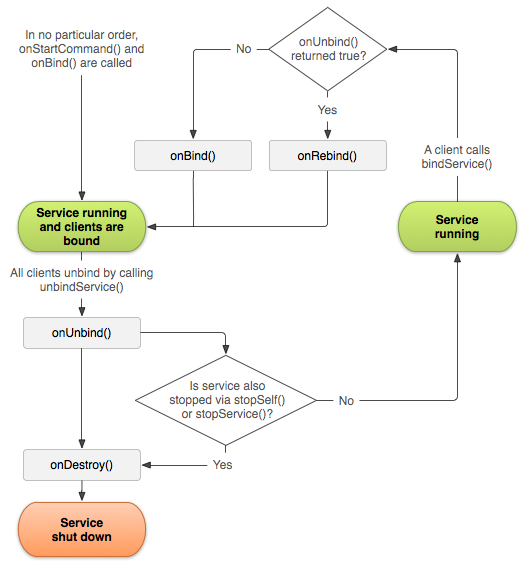
\includegraphics[scale=0.5]{service-binding-tree-lifecycle}\\
이 그림에서 마름모꼴 분기점은 Started \& Bound Service의 경우인데, 앞에서 얘기했듯이 가능하면 생각하지 않는 것이 좋다.\\

기본적으로 Bound Service에서 bindService()를 실행한 클라이언트가 모두 unbindService()를 호출한다면, Service에서는 onUnbind()가 호출되고 onDestroy()까지 호출된다.
Activity에서 Bound Service를 사용할 때는 onStart()와 onStop()에서 bindService()와 unbindService()를 각각 호출하는 것을 권장하고 있다. unbindService()를 실행 시에 연결되어 있는 클라이언트 수가 0가 되면 Service는 종료될 수 있음을 생각해보자. onResume/onPause에서 bind/unbind 하는 경우 onResume/onPause는 빈번하게 트랜지션이 일어나는데(전원 버튼 누르기, 다이얼로그 테마 Activity를 위에 띄우기 등) onPause()를 통해 unbindService()가 실행되고 Service가 종료될 수도 있다. 
그리고서 onResume()에서 다시 시작해야만 한다. 종료된 Service라면 다시 생성하는 비용이 들게 되는데 빈번한 트랜지션에서 계속 생성/종료하는 것은 적합하지 않다.\\

bindService()를 통해 Bound되었으면 이제는 호출하는 쪽과 호출되는 쪽은 클라이언트-서버 관계로 파악하면 된다. 클라이언트에서 메서드를 호출하면 Service에서 결과를 리턴하는 방식이다. 
조회해서 결과를 리턴한다면 떠올려지는 게 바로 ContentProvider이다. 로컬 바인딩은 타입을 자유롭게 쓸 수 있으므로 크게 고민하지 않아도 되겠지만, 리모트 바인딩의 경우는 ContentProvider를 대신 쓸 수도 있다. 물론 DB에서 가져오는 값이 아닐 때는 Cursor 타입으로 리턴하도록 조작해야 한다.\\

얘기가 나온 김에 ContentProvider를 써서 동일한 기능을 만들어보자.
\begin{lstlisting}[frame=single]
	@Override
	public Cursor query(Uri uri, String[] projection, String selection, String[] selectionArgs, String sortOrder) {
		...
		switch (URI_MATCHER.match(uri)) {
			...
			case VALID_CALENDAR:
				return validCalendar(Long.parseLong(selectionArgs[0]), 
					CalendarType.valueOf(selectionArgs[1]));
				
		}
		throw new IllegalArgumentException("Unknown URI " + uri.toString());
	}

	private Cursor validCalendar(long calendarId, CalendarType calendarType) {
		Calendar calendar = null;
		if (calendarType == CalendarType.NORMAL) {
			...
		} else {
			...
		}
		MatrixCursor cursor = new MatrixCursor(new String[] {"calendar"}); // (1)
		if (calendar != null) {
			cursor.newRow().add("valid");
		}
		return cursor;
	}
\end{lstlisting}
21라인(1)에서 DB Cursor가 아니고 직접 Cursor에 값을 채우는 방법으로 MatrixCursor를 사용하였다.\\

클라이언트에서는 아래와 같이 사용한다.
\begin{lstlisting}[frame=single]
	public boolean isValidCalendar(long calendarId, CalendarType type) {
		Cursor cursor = contentResolver.query(Uri.withAppendedPath(CONTENT_URI, 
			"valid_calendar"), null, null, 
			new String[] {String.valueOf(calendarId), type.name()}, null);
		return (cursor.getCount() > 0);
	}
\end{lstlisting}

Service에서도 작업이 오래 걸린다면 백그라운드 스레드에서 작업을 실행하는 것을 고려할 수 있다. 이때는 네 가지 방법을 고려할 수 있다.
\begin{itemize}
\item 스레드 작업이 끝났을 때 sendBroadcast() 메서드를 통해서 데이터를 전달하거나, 데이터가 많은 경우 다시 클라이언트가 폴링해서 데이터를 가져올 수도 있다.
\item Binder Callback을 메서드에 파라미터로 전달해서 결과를 받는 방법도 있다.\footnote{ApiDemos에서 RemoteService를 참고하자.} 이 방법은 안드로이드 프레임워크에서 많이 쓰이는 방법이다. 앞에 얘기했듯이 Toast.show() 메서드에서도 쓰이고, Activity, Service 등의 컴포넌트 생명주기가 불려지는 것도 system\_server 프로세스의 ActivityManagerService에서 Binder Callback을 통해서 호출된다(ActivityThread의 내부 클래스인 ApplicationThread가 바로 Binder Callback이다).
\item bindService() 메서드의 파라미터인 Intent에 ResultReceiver를 전달하여 Service의 onBind()에서 ResultReciever를 가져오고 작업을 실행하며 결과를 클라이언트에 전달한다.
\item Messenger를 통해서 양방향 통신을 할 수 있다. Messenger도 내부적으로 Binder Callback을 사용하고 있다. Messenger에 대해서는 별도의 절에서 살펴보자.
\end{itemize}

\subsection{Messenger}
\label{subsec:messenger}
Messenger는 Binder Callback을 내부적으로 래핑해서 Bound Service와 클라이언트 간에 Handler로 메시지를 보내고 처리하는 방식을 제공한다.
필자는 수년 간 앱을 개발하면서 Messenger를 사용한 케이스를 몇 번 보지 못했다. 
앞에서 살펴보았듯이 Service와 다른 컴포넌트 간 통신은 다른 옵션으로도 가능하기 때문이다. 
하지만 Messenger를 알아두면 다른 옵션을 복잡하게 사용하지 않아도 된다. 알아두고 필요할 때 활용하도록 하자.\\

먼저 Messenger의 기본적인 내용을 알아보자. 
\begin{itemize}
\item Messenger는 Parcelable 인터페이스를 구현해서 프로세스 간에 전달할 수 있는 객체이다.
\item Messenger에는 2개의 생성자가 있다. Messenger(Handler target)는 Handler를 감싼 것으로 클라이언트와 Bound Service 양쪽에 있다. Messenger(IBinder target)는 Binder Proxy를 생성하는 것으로 클라이언트에 있다.
\item aidl을 내부적으로 사용하는데 IMessenger 인터페이스로 되어 있다. 
이름만으로 보면 Messenger가 IMessenger.Stub을 구현할 것 같은데 그렇지 않고, Handler의 내부 클래스인 MessengerImpl에서 IMessenger.Stub을 구현하고 있다. Stub에서는 Handler의 sendMessage() 메서드를 호출하기만 한다.
\item \ref{sec:messagequeue}절의 Message 소스를 보면 replyTo라는 public 변수가 있다. Handler에 Message를 보내면서 응답을 받을 곳을 replyTo에 지정할 수 있다.
\item Messenger의 send() 메서드는 결과적으로 Binder 통신을 통해 Stub의 메서드를 호출한다. 리모트 통신이기 때문에 send() 메서드는 RemoteException을 던질 수 있다. 
\end{itemize}

%http://developer.android.com/intl/ko/reference/android/app/Service.html
이제 날씨 정보를 업데이트하는 기능을 Messenger로 만들어보자. 요구 사항은 이렇다.
\begin{itemize}
\item 처음 Activity에서 bindService()를 하면, Bound Service에서 날씨 정보를 가져오고 내부에서 주기적으로(예제에서는 1분) 날씨 정보를 가져온다.
\item 날씨 정보를 가져올 때마다 Bound된 Activity에 정보를 전달해서 화면에 보여준다.
\item 추가로 클라이언트가 Bound되면 최신 날씨 정보를 클라이언트에 전달한다.
\item 화면에는 [Refresh] 버튼이 있어서 이 버튼을 클릭하면, 날씨 정보를 새로 가져오고 Bound된 클라이언트 모두에 날씨 정보를 새로 전달한다.
\end{itemize}

Service 코드를 먼저 살펴보자.
\begin{lstlisting}[frame=single]
public class MessengerService extends Service {

	/* input message */
	public static final int MSG_REGISTER_CLIENT = 1;
	public static final int MSG_UNREGISTER_CLIENT = 2;
	public static final int MSG_REFRESH = 3;

	/* output message */
	public static final int MSG_WEATHER = 11;

	public static final String WEATHER_TEXT = "weatherText";
	public static final String TEMPERATURE = "temperature";

	private final ScheduledExecutorService scheduler 
		= Executors.newScheduledThreadPool(1); // (1)

	private ArrayList<Messenger> clients = new ArrayList<>(); // (2)

	private Bundle lastData;

	private class IncomingHandler extends Handler { // (3)

		@Override
		public void handleMessage(Message msg) {
			switch (msg.what) {
				case MSG_REGISTER_CLIENT:
					clients.add(msg.replyTo); // (4)
					if (lastData != null) { // (5)
						Message message = Message.obtain(null, MSG_WEATHER);
						message.setData(lastData);
						try {
							msg.replyTo.send(message);
						} catch (RemoteException e) {
						}
					}
					break;
				case MSG_UNREGISTER_CLIENT:
					clients.remove(msg.replyTo); // (6)
					break;
				case MSG_REFRESH:
					scheduledFuture.cancel(true); // (7)
					fetchWeather();
					break;
				default:
					super.handleMessage(msg);
			}
		}

	}

	private Messenger messenger = new Messenger(new IncomingHandler()); // (8)
	private ScheduledFuture scheduledFuture;

	@Override
	public void onCreate() {
		super.onCreate();
		fetchWeather(); // (9)
	}

	private void fetchWeather() {
		scheduledFuture = scheduler.scheduleAtFixedRate(new Runnable() {

				@Override
				public void run() { // (10)
					Weather weather = callWeatherAPI(); // HTTP Call
					Message message = Message.obtain(null, MSG_WEATHER);
					Bundle bundle = message.getData();
					bundle.putString(WEATHER_TEXT, weather.weatherText]);
					bundle.putInt(TEMPERATURE, weather.temparature));

					lastData = new Bundle(bundle); // (11)
					for (int i = clients.size() - 1; i >= 0; i--) {
						try {
							clients.get(i).send(message);
						} catch (RemoteException e) {
							clients.remove(i); // (12)
						}
					}
				}

			}, 0, 1, TimeUnit.MINUTES); // (13)
	}

	@Override
	public IBinder onBind(Intent intent) { // (14)
		return messenger.getBinder();
	}

}
\end{lstlisting}
\begin{itemize}
\item 4$\sim$6라인은 클라이언트에서 들어오는 Message의 what에 해당하는 값이고, 9라인은 클라이언트에 보내는 Message의 what에 해당하는 값이다.
\item 57라인(9)에서 바로 날씨 정보를 가져온다. 첫 번째 클라이언트가 bindService()를 호출하면 이때 onCreate()가 호출되고 곧바로 날씨 정보를 가져오겠다는 의미이다.
\item 15라인(1)에서 스레드 개수가 1개인 ScheduledThreadPoolExecutor을 생성한다. 81라인(13)의 파라미터를 보면 즉시 태스크를 실행하고 그 이후에는 1분마다 실행한다.
\item 17라인(2)에서 클라이언트 Messenger 목록을 clients 변수에 유지한다.
\item 21라인(3)의 Handler는 클라이언트에서 들어오는 Message를 처리하는 용도이다.
\item 51라인(8)에서 Handler를 감싼 Messenger를 생성하고, 이것을 85라인(14)의 onBind() 메서드에서 messenger.getBinder()로 클라이언트에 전달한다.
\item 27라인(4)에서 MSG\_REGISTER\_CLIENT 값이 들어오면 replyTo에 전달되는 Messenger를 클라이언트 목록에 추가한다.
\item 64라인(10)의 Runnable Task에서는 날씨 정보를 가져와서 Bundle에 담고서 클라이언트 목록에 send() 메서드로 전달한다. foreach 문을 사용하지 않고 인덱스가 높은 숫자부터 쓴 이유는 클라이언트가 dead 상태인 경우에 RemoteException이 발생하는데 76라인(12)에서 클라이언트 목록에서 해당 클라이언트를 제거해도 문제가 없게 하려는 것이다.
\item 71라인(11)에 lastData에 최신 값을 저장하고서, 28라인(5)에서 이 값이 있다면 새로 등록한 클라이언트에 전달한다. 이 방식을 사용하는 이유는 아직 갱신주기가 되지 않은 경우, 최대 1분동안 새로 Bound된 클라이언트에서는 날씨 정보를 전달받을 수 없기 때문이다.
\item 38라인(6)에서 MSG\_UNREGISTER\_CLIENT 값이 들어오면 클라이언트 목록에서 제거한다.
\item 41라인(7)에서 MSG\_REFRESH 값이 들어오면 기존 ScheduleFuture를 취소하고 새로 날씨 정보를 가져온다.
\end{itemize}

이제 클라이언트 코드를 보자.
\begin{lstlisting}[frame=single]
public class MessengerActivity extends Activity {

	private class IncomingHandler extends Handler { // (1)
		@Override
		public void handleMessage(Message msg) {
			switch (msg.what) {
				case MessengerService.MSG_WEATHER:
					Bundle bundle = msg.getData();
					weather.setText(bundle.getString(
						MessengerService.WEATHER_TEXT) + ", Temparature: " 
						+ bundle.getInt(MessengerService.TEMPERATURE));
					break;
				default:
					super.handleMessage(msg);
			}
		}
	}

	private Messenger outMessenger;

	private ServiceConnection serviceConnection = new ServiceConnection() {

		@Override
		public void onServiceConnected(ComponentName className, 
				IBinder service) { // (2)
			outMessenger = new Messenger(service);
			try {
				Message msg = Message.obtain(null,
					MessengerService.MSG_REGISTER_CLIENT);
				msg.replyTo = inMessenger;
				outMessenger.send(msg); // (3)
			} catch (RemoteException e) {
			}
			Toast.makeText(MessengerActivity.this, "Connected.",
				Toast.LENGTH_SHORT).show();
		}

		@Override
		public void onServiceDisconnected(ComponentName className) {
			outMessenger = null;
			Toast.makeText(MessengerActivity.this, "Disconnected.",
				Toast.LENGTH_SHORT).show();
		}

	};

	private Messenger inMessenger = new Messenger(new IncomingHandler()); // (4)

	private TextView weather;

	@Override
	protected void onCreate(Bundle savedInstanceState) {
		super.onCreate(savedInstanceState);
		setContentView(R.layout.two_buttons);
		weather = (TextView) findViewById(R.id.title);
	}

	@Override
	protected void onStart() {
		super.onStart();
		bindService(new Intent(this, MessengerService.class), serviceConnection,
			Context.BIND_AUTO_CREATE);
	}

	@Override
	protected void onStop() {
		super.onStop();
		if (outMessenger != null) {
			try {
				Message msg = Message.obtain(null,
					MessengerService.MSG_UNREGISTER_CLIENT);
				msg.replyTo = inMessenger;
				outMessenger.send(msg);
			} catch (RemoteException e) {
			}
		}
		unbindService(serviceConnection);
	}

	public void onClickRefresh(View view) { // (5)
		Toast.makeText(MessengerActivity.this, "Refresh.",
			Toast.LENGTH_SHORT).show();
		if (outMessenger != null) {
			try {
				Message msg = Message.obtain(null, 
					MessengerService.MSG_REFRESH);
				msg.replyTo = inMessenger;
				outMessenger.send(msg);
			} catch (RemoteException e) {
			}
		}
	}

}
\end{lstlisting}
\begin{itemize}
\item \ref{subsec:binding_special}절에서 얘기한 가이드대로 onStart()와 onStop() 메서드에서 bindService()와 unbindService() 메서드를 호출한다.
\item 3라인(1)의 Handler는 클라이언트에 전달되는 Message를 처리하는 용도이다. 이것을 감싼 Messenger를 47라인(4)에서 outMessenger로 생성한다.
\item 25라인(2)의 onServiceConnnected() 콜백 안에서는 IBinder를 감싼 Messenger를 생성하고 replyTo에는 inMessenger를 대입해서 31라인(3)에서 Service에 등록하라는 Message를  보낸다.
\item 80라인(5)은 [Refresh] 버튼을 클릭할 때 동작이다. Service에 날씨 정보를 갱신하라는 Message를 보낸다.
\end{itemize}

이 샘플을 통해 Bound Service를 사용하는 한 가지 장점을 알 수 있다. 각 클라이언트에서 네트워크를 통한 API 호출을 매번 하지 않고 Service 한 곳에서만 네트워크 통신을 하고 모든 클라이언트에 결과를 반영할 수 있는 구조가 가능하다. 샘플처럼  Messenger를 이용하면 더 단순해진다.
% http://wikiware-textcube.blogspot.com/2009/12/4-%EC%95%88%EB%93%9C%EB%A1%9C%EC%9D%B4%EB%93%9C-%EC%96%B4%ED%94%8C%EB%A6%AC%EC%BC%80%EC%9D%B4%EC%85%98-%EA%B8%B0%EC%B4%88.html
